\documentclass[a4paper]{article}

\usepackage{fullpage, amsmath, amssymb, verbatim} % Package to use full page
\usepackage{graphicx}

\title{Deep Learning: Assignment One}
\author{Aditi Nair (asn264) and Akash Shah (ass502)}
\date{March 7, 2017}
\begin{document}

\maketitle

\section{Backprop}
\begin{enumerate}
\item{ \textbf{Nonlinear Activation Functions}
\newline
\newline
\textbf{SIGMOID:}
\newline
\newline
The sigmoid function can be expressed as:
$$x_{out} = \frac{1}{1 + e^{-x_{in}}} = \frac{1}{1 + e^{-x_{in}}} \cdot \frac{e^{x_{in}}}{e^{x_{in}}} = \frac{e^{x_{in}}}{1+e^{x_{in}}} $$
Then it follows that:
$$\frac{\delta x_{out}}{\delta x_{in}} = \frac{(1+e^{x_{in}} )e^{x_{in}} - (0 + e^{x_{in}})e^{x_{in}}  } {(1+e^{{x_{in}}})^2} 
= \frac{e^{x_{in}} + e^{2x_{in}} - e^{2x_{in} }} {(1+e^{x_{in}})^2} =  \frac{e^{x_{in}} } {(1+e^{x_{in}})^2} 
$$
Finally:
$$\frac{\delta E} {\delta x_{in}} = \frac{\delta E}{\delta x_{out}} \cdot  \frac{\delta x_{out}}{\delta x_{in}}
= \frac{\delta E}{\delta x_{out}} \cdot \frac{e^{x_{in}}}{(1+e^{x_{in}})^2}$$
\newline
\textbf{TANH:}
\newline
\newline
The hyperbolic tangent function can be expressed as:
$$x_{out} = \frac{exp(2x_{in})-1}{exp(2x_{in})+1}$$
Then it follows that:
$$ \frac{\delta x_{out}}{\delta x_{in}} = \frac{ ( exp(2x_{in})+1 )(2exp(2x_{in})) - (2exp(2x_{in}))(exp(2x_{in})-1)  }{ (exp(2x_{in})+1)^2 } $$
$$ = \frac{ 2exp(4x_{in})+2exp(2x_{in})-2exp(4x_{in})+2exp(2 x_{in}) }{ (exp(2x_{in})+1)^2 } $$
$$ = \frac{ 4 exp(2 x_{in}) }{(exp(2x_{in})+1)^2 }$$
Finally:

$$\frac{\delta E}{\delta x_{in}} = \frac{\delta E}{\delta x_{out}} \cdot  \frac{\delta x_{out}}{\delta x_{in}} =  \frac{\delta E}{\delta x_{out}} \cdot \frac{4 exp(2 x_{in})}{(exp(2 x_{in})+1)^2} $$
\newline
\textbf{RELU:}\newline
\newline
The RELU function can be expressed as:
$$x_{out} = max(0,x_{in})$$
It follows that:
\begin{equation}\frac{\delta x_{out}}{\delta x_{in}} = 
\left\{
	\begin{array}{ll}
		1 & \mbox{if } x_{in}  > 0\\
		0 & \mbox{otherwise}
	\end{array}
\right.\end{equation}
When we write $x_{in} = x_{in}^+ - x_{in}^-$, we can rewrite this as:
$$\frac{\delta x_{out}}{\delta x_{in}} = sign(x_{in}^+) $$ 
Therefore:
$$\frac{\delta E}{\delta x_{in}} =  \frac{\delta E}{\delta x_{out}} \cdot \frac{\delta x_{out}}{\delta x_{in}} = \frac{\delta E}{\delta x_{out}} \cdot sign(x_{in}^+) $$

}

\item{ \textbf{Softmax} 
\newline
\newline
We can express the softmax function as:

$$p(y=i|x_{in}) = (x_{out})_i = \frac{e^{- \beta (x_{in})_i }}{ \sum_k e^{- \beta (x_{in})_k } }$$

If $i \neq j$, then the numerator is constant with respect to $(x_{in})_j$. In this case, we write:
$$\frac{\delta (x_{out})_i}{ \delta (x_{in})_j } 
= e^{- \beta (x_{in})_i} \cdot -1 \cdot  \Big( \sum_k e^{- \beta (x_{in})_k} \Big)^{-2} \cdot - \beta e^{- \beta (x_{in})_j } $$
$$ = \frac{\beta e^{-\beta ( (x_{in})_i + (x_{in})_j )}}{ \Big( \sum_k e^{- \beta (x_{in})_k} \Big)^2} $$

If $i = j$, then we write:
$$\frac{\delta (x_{out})_i}{ \delta (x_{in})_j } = \frac{\delta (x_{out})_i}{ \delta (x_{in})_i } $$
$$ = \frac{ (-\beta e^{-\beta (x_{in})_i } ) \Big( \sum_k e^{- \beta (x_{in})_k} \Big) - (e^{-\beta (x_{in})_i )}) ( - \beta e^{-\beta (x_{in})_i  })}{\Big( \sum_k e^{- \beta (x_{in})_k} \Big)^2}$$
$$ = \frac{ - \beta e^{- \beta (x_{in})_i }  \Bigg[ \Big( \sum_k e^{- \beta (x_{in})_k} \Big) - e^{-\beta (x_{in})_i}  \Bigg] } {\Big( \sum_k e^{- \beta (x_{in})_k} \Big)^2 } $$

}
\end{enumerate}

\section{Techniques}
\subsection{Optimization}

\textbf{Gradient Descent Step by Momentum Method:}
$$v_{t+1} = \mu v_t - \epsilon \nabla f(\theta_t) $$
$$\theta_{t+1} = \theta_t + v_{t+1}$$

$f(\theta)$ is an object function we are trying to minimize. $\epsilon > 0$ is the learning rate, $\mu \in [0,1]$ is the momentum coefficient and $v_t$ is the velocity vector.  
\newline
\newline
\textbf{Gradient Descent Step by Nesterov's Accelerated Gradient (NAG) Method:}
$$v_{t+1} = \mu v_t - \epsilon \nabla f(\theta_t + \mu v_t) $$
$$\theta_{t+1} = \theta_t + v_{t+1}$$
\textbf{Comparison of Methods:}
\newline
\newline
In both methods, the previous velocity is decayed by $\mu$, and then we apply a ``correction" to it based on the gradient of $f$. The momentum method computes the gradient update based on the value of $\nabla f$ at $\theta_t$ whereas the NAG method computes the correction based on the value at $\theta_t + \mu v_t$, which looks like $\theta_{t+1}$ without the gradient-based correction. The NAG method is helpful in situations where $\mu v_t$ is a suboptimal update direction for $\theta_{t+1}$, since in this case $\nabla f(\theta_t + \mu v_t) $ will point more strongly to $\theta_t$. In comparison, the momentum method would have to take the step incorporating $\mu v_t$ and then correct the step later. Compounded over time, this allows NAG to prevent divergence.

\subsection{Reducing Overfitting}

\begin{enumerate}
\item{ Ideally we could have an ensemble of independently-trained weak or shallow neural networks whose results we could combine to get a more robust model. Since this is infeasible due to the computational burden of training neural networks and the limited availability of labelled data, we approximate having a larger number of less complex neural nets by applying dropout, in which we choose to randomly and independently drop units from a network with some probability. When we encounter a new training point or batch, we essentially train it on a new ``thinned" network corresponding to the currently non-dropped network units. Each ``thinned" network gets trained relatively few times, effectively creating a weak learner. At test time, we do not apply dropout, so we essentially combine the results of each ``thinned" network. This is like an ensemble method, in that we create many weak learners and then combine their output at test time. 

 }
\item{Let $x_i$ be a unit in the hidden layer of a neural network. By applying dropout with a ``keep" probability of $p$, the expected value of $x_i$ at train time can be expressed as:
$$\mathbb{E}[x_i] = p \cdot x_i + (1-p) \cdot 0 = p x_i   $$
However, at test time, if we do not apply dropout and do not scale the values propagated from the unit $x_i$, the expected value will be:
$$\mathbb{E}[x_i] = 1 \cdot x_i = x_i   $$
Now, on average, the values propagated from this unit will be very different from those encountered during training and the final probability scores of our model at test time will be distorted by this change. This effect will be exacerbated by the fact that dropout is generally applied to all or many of the units in the hidden layer. Therefore, we need to scale the outgoing weights of $x_i$ by $p$ at test time so that the expected value at test time equals the expected value at train time:
$$\mathbb{E}[x_i] = p \cdot x_i = p x_i   $$

}
\item{Common data augmentation methods, which increase the size of the training set by transforming the original data, include: 
\begin{itemize}
\item{Rotationed, translated and zoomed-in or zoomed-out versions of the original images.}
\item{Stretched or squeezed versions of the original images.}
\item{Horizontally or vertically reflected versions of the original images}
\item{Elastic distortions of the original image, which is a type of image distortion that mimics natural oscillations in handwriting.}
\end{itemize}

Of the methods listed above, all of them would be appropriate for the MNIST dataset except for horizontal or vertical reflections, as a vertically reflected 2 could look like a 5, and horizontally reflected digits would not be classified as the same digit by humans. Also, one thing to keep in mind with rotation is that we must limit the rotation degree as a 9 rotated more than 90$^{\circ}$ or less than -90$^{\circ}$ would look more like a 6 than a 9.

}
\end{enumerate}

\subsection{Initialization}
\begin{enumerate}
\item{ We need to be careful about how we initialize weights in a neural network. If the weights of a matrix/vector are too small, then the signal will ``shrink" as it passes through these units. If they are too big, the signal may explode and learning will diverge. For this reason, we rely on initialization methods to start off the weights at a safe range. 
\newline
\newline
In Xavier initialization, we choose $w_{ij}$ in a weight matrix $W$ from uniform (or Gaussian) distribution with $\mu=0$ and $\sigma^2 = \frac{1}{n_i}$ where $n_i$ is the number of input neurons to the corresponding unit. Analogously, we would also want $\sigma^2 = \frac{1}{n_o}$ where $n_o$ is the number of output neurons to the corresponding unit. In order to satisfy these simulatanously, Xavier et al. sugguests an initialization strategy of $\sigma^2 = \frac{1}{n_i + n_o}$ Generally, this initialization ensures that the variance of the input gradient and output gradient are the same in networks using non-linearities like the sigmoid and hyperbolic tangent functions.
\newline
\newline
However, since the authors of the Xavier method derived the parameters for the distribution of $W_{ij}$ based on properties of the sigmoid and hyperbolic tangent function, this is not necessarily well-suited for networks using RELU units, whose gradients generally behave very differently. Based on properties of the RELU unit, He et al. recommend choosing $w_{ij}$ from a Gaussian distribution with $\mu=0$ and $\sigma^2=\frac{2}{n_i}$. 

}
\item{ The VGG team first trained a small, shallow network. Next, they trained a deeper network where the first four and last three layers of the network were initialized with the trained weights from the first shallow model. These weights were allowed to change during the training procedure, and other weights in the deeper model were randomly initialized. 
\newline
\newline 
Coate et al. used the following procedure to extract features from unlabelled data: first, they applied some basic preprocessing (like normalization) to the unlabelled data. Next they extracted ``patches" from the images and developed vector representations of these patches using unsupervised methods like sparse auto-encoders, RBMs, K-Means, etc. Finally, they extracted the same-sized patches from the labelled images and applied the same unsupervised methods to the patches to get vector representations of the labelled patches. Assuming the unsupervised methods return feature vectors in $\mathbb{R}^k$, the resulting feature vectors were treated as a new image representations with $k$ channels. After performing pooling on the quadrants of each channel, the authors were able to develop a final feature vector of length $4k$. 

\subsection*{FINAL MODEL CONFIGURATION: EXPERIMENTS AND RESULTS}
- Also need to explain final model architecture and configuration (include stopping criterion, optimizer and batch sizes for all experiments).
\newline
\newline
\textbf{Section 2 Methods for Improving Accuracy:}
\newline
\newline
Our model uses Nesterov's Accelerated Gradient (NAG) method, dropout, Xavier initialization, and data augmentation to improve accuracy. Below we provide a short summary of the results of experiments using these methods. 

\begin{center}
\begin{tabular}{ |c|c|c| } 
 \hline
 Model & Train Accuracy & Validation Accuracy \\ \hline
 Baseline (with NAG and Dropout) & 97.83 & 95.12 \\ 
 Baseline + Xavier & 97.90 & 95.78 \\ 
 Baseline + Xavier + Data Augmentation & 98.90 & 97.08 \\ 
 \hline
\end{tabular}
\end{center}

Below, we show the training and validation curves for a baseline model trained using the NAG method as well as dropout, which were both implemented in the provided starter code. (The NAG method is built into the SGD optimizer in PyTorch, and can be used by modifying the momentum parameter appropriately.)

\begin{figure}
  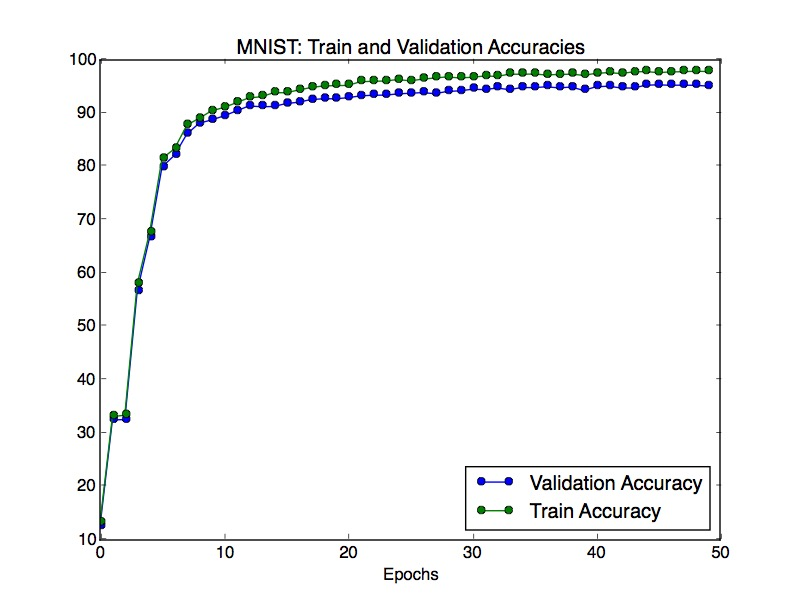
\includegraphics[width=12cm]{../plots/accuracies_baseline.jpg}
  \centering
  \caption{Baseline.}
  \label{fig:boat1}
\end{figure}

Next, we applied initialization from the Xavier/He papers with $\sigma^2 = \frac{1}{n_i + n_o}$ for fully connected network modules, and $\sigma^2 = \frac{1}{n_i}$ for convolutional layers. As the number of input and output neurons for fully connected layers are readily accessible, we went with the Xavier initialization for them while using He initialization for the convolutional layers. The training and validation curves for our baseline model plus Xavier initialization is shown below.

\begin{figure}
  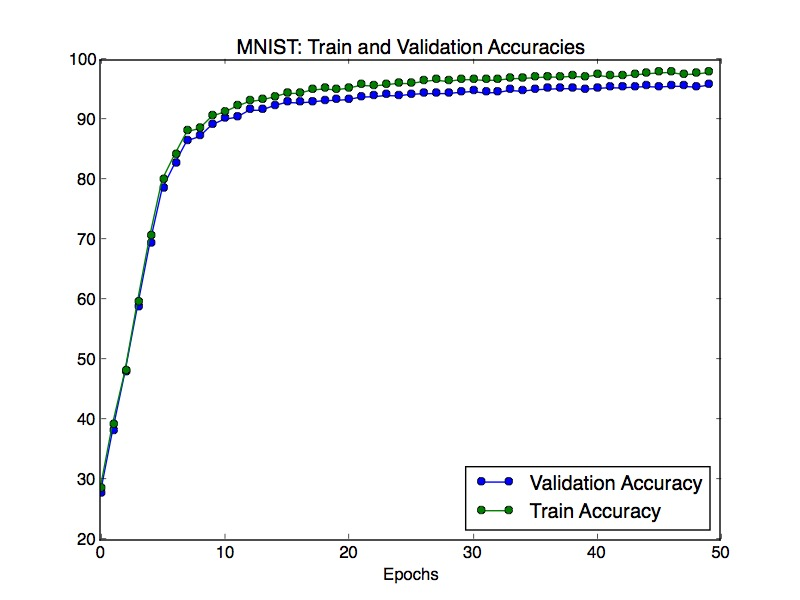
\includegraphics[width=12cm]{../plots/accuracies_xavier.jpg}
  \centering
  \caption{Baseline + Xavier Initialization}
  \label{fig:boat1}
\end{figure}

Finally, we applied data augmentation to the dataset. Our data augmentation process was done offline, so the train set was enchanced before we started training. We first added a rotated version of the image, where the rotation parameter was between -45 and 45 degrees. Then, we added a translated version of the image, where both the x and y coordinates were translated by a random number of pixels between -2 and 2. Next, we added a zoomed in/out version of the image by randomly picking to zoom in or zoom out, and then choosing a scaling coefficient between 1 and 2. The last data augmentation method we used was elastic distortion. The parameters were randomly chosen in the following ranges $\sigma \in (5,6)$ and $\alpha \in (36,38)$ as suggested by Ciresan et al. in ``Handwritten Digit Recognition with a Committee of Deep Neural Nets on GPUs".
\newline
\newline
Surprisingly, we noticed that the model accuracy on the augmented training set was significantly lower than the model accuracy on the validation set. For this reason, we also evaluated the model accuracy on the original, un-augmented training set (shown in blue in the graph below), which behaves as expected in comparison to the model accuracy on the validation set. We surmised that model performance on the augmented dataset was poor compared to performance on the original training and validation sets because the classification task on the augmented dataset was significantly harder. In the augmented dataset, there is most likely a higher proportion of images which are difficult to classify - those that are rotated, zoomed, or otherwise distorted in a manner that might be uncommon in natural human writing - and which are accordingly infrequent in the un-augmented training and validation sets. 

\begin{figure}
  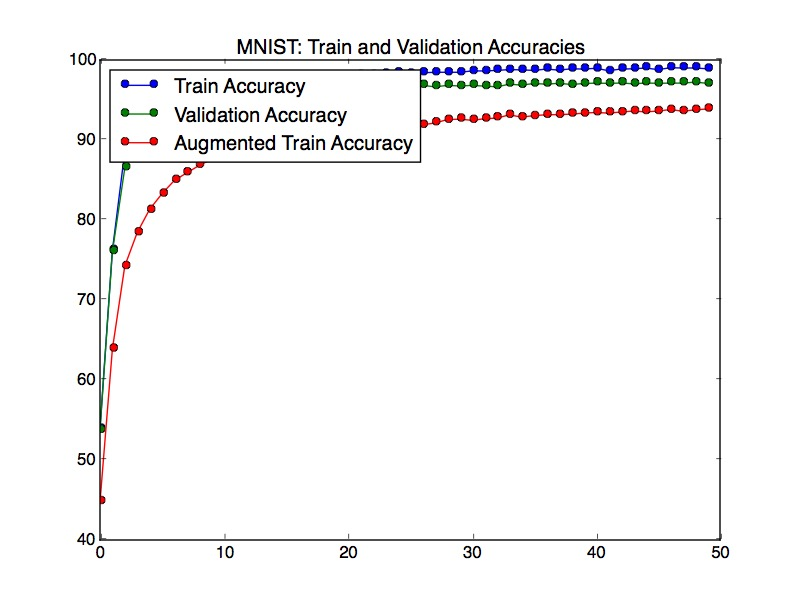
\includegraphics[width=12cm]{../plots/accuracies_augmented.jpg}
  \centering
  \caption{Baseline + Xavier Initialization + Data Augmentation}
  \label{fig:boat1}
\end{figure}

\textbf{Unsupervised Methods for Improving Accuracy:}
\newline
\newline
In order to incorporate unlabelled MNIST data into our models, we relied on the pseudo-label method described by Dong-Hung Lee in ``Pseudo-Label : The Simple and Efficient Semi-Supervised Learning Method for Deep Neural Networks". In the pseudo-label method, supervised learning models are trained using labelled and unlabelled data simultaneously. The unlabelled data is given a provisory label based on the model's latest prediction for that data. The weight of the unlabelled data in the objective function is annealed over time such that more powerful versions of the model attribute greater weight to unlabelled data and provisory labels. 
\newline
\newline
Therefore we trained our model on the following objective function:
$$L = \frac{1}{N} \sum_{m=1}^{N} NLL(y_m, \hat{y_m}) + \alpha(t) \frac{1}{N'} \sum_{m=1}^{N'} NLL(y_m, \hat{y_m}) $$
Above, the first summand computes the average negative log likelihood over all labelled samples. The second summand computes the average negative log likelihood over all unlabelled samples and their pseudo-labels. $\alpha(t)$ is an annealing function which is computed as:
\begin{equation}\alpha(t) = 
\left\{
	\begin{array}{ll}
		0 & \mbox{if } t <T_1\\
		\frac{t-T_1}{T_2-T_1} \alpha_f & \mbox{if } T_1 \leq t < T_2 \\
		\alpha_f & \mbox{if } T_2 \leq t
	\end{array}
\right.\end{equation}
Above, $t$ refers to current training epoch. $T_1$ and $T_2$ are thresholds which determine the inclusion and weighting of the pseudo-labels over time. Before $T_1$, pseudo-labels are effectively ignored - so higher values of $T_1$ will ideally force the model to refrain from using pseudo-labels until the model is at least somewhat adept at guessing most labels. Once $t \geq T_2$, depending on the choice of the weighting constant $\alpha_f$, the unlabelled data can be weighted significantly more heavily than the original labelled data. Between $T_1$ and $T_2$ the weight of unlabelled data is increased as $t$ increases. 
\newline
\newline
In our experiments we set $T_1 = ??$, $T_2 = ??$ and $\alpha_f = ??$. The original author updated the pseudo-labels after every optimization step in a gradient step procedure. However, we surmised that since our batch sizes are relatively small, and the loss surface was non-convex, individual gradient steps were likely to be noisy. Therefore, we waited a full epoch before updating the pseudo-labels - hopefully averaging away the noise in individual gradient steps. 
\newline
\newline

[INSERT PLOT, ACCURACY RESULTS, AND PARAMETER DETAILS]
}
\end{enumerate}
\end{document}
